\documentclass[conference]{IEEEtran}
\IEEEoverridecommandlockouts
\usepackage{cite}
\usepackage{amsmath,amssymb,amsfonts}
\usepackage{algorithmic}
\usepackage{graphicx}
\usepackage{textcomp}
\usepackage{xcolor}
\usepackage{url}
\usepackage{booktabs}
\usepackage[hidelinks]{hyperref}

\begin{document}

\title{Human Activity Recognition from Wrist-Worn Accelerometers\\
{\footnotesize NYCU Data Mining, Assignment 3, 2026 Spring}
}

\author{\IEEEauthorblockN{Student ID: 314540061}}

\maketitle

\begin{abstract}
This report describes my solution to the Assignment~3 Human Activity Recognition
(HAR) Kaggle competition, in which each five-minute wrist-accelerometer recording
must be classified into one of six activities. My final system is a six-model
ensemble of gradient-boosted trees (LightGBM, XGBoost, CatBoost) and a multi-layer
perceptron on 334 hand-crafted features, together with a CNN--LSTM and a ROCKET
model on the raw signal, combined by a hill-climbing weighted blend and a per-class
decision-threshold correction. It reaches a public-leaderboard macro-F1 of
\textbf{0.8267}, comfortably above the Baseline-3 target of 0.7088. All code is
available at GitHub:~\href{https://github.com/Lappykentang/DM2026-Assignment-3}{\color{blue}https://github.com/Lappykentang/DM2026-Assignment-3}.
\end{abstract}

\section{Preliminary Analysis}
\textbf{Data.} The dataset~\cite{bruno2014public} consists of accelerometer
recordings from 100 users. Each file is a five-minute window already aggregated to
300 one-second rows with six columns: the per-second mean acceleration on each axis
(\texttt{mean\_x}, \texttt{mean\_y}, \texttt{mean\_z}) and the within-second standard
deviation (\texttt{std\_x}, \texttt{std\_y}, \texttt{std\_z}); every file has exactly
one activity label in $\{0,\dots,5\}$. The training set contains 11{,}020 files from
60 users and the test set 6{,}849 files from a \emph{disjoint} 40 users.

\textbf{Observations that shaped the design.} Three facts drove every later
decision. (i) Every file is exactly 300 rows with no missing values, so no
variable-length or imputation handling is needed. (ii) The train and test users do
not overlap, so a random file-level split would leak user identity and inflate
validation scores; I therefore use \texttt{GroupKFold} by \texttt{user\_id}
everywhere, which validates only on unseen users and mirrors the real train/test
gap. (iii) The classes are highly imbalanced (Fig.~\ref{fig:dist}): classes~0 and~1
are about 42\% of files each, whereas class~2 is only 3.2\%, class~4 1.3\%, and
class~5 4.8\%. Because the metric is macro-F1, the rare classes count as much as the
frequent ones, and in practice the rare class~2 is where almost all of the error
concentrates. A further physical note from the assignment is useful: the sensor is
worn on the wrist, the readings are in units of $g$, and the gravity component has
\emph{not} been removed---so the mean channels carry a user-dependent orientation
offset, while the std channels reflect only motion intensity and are therefore far
more comparable across users.

\begin{figure}[t]
\centering
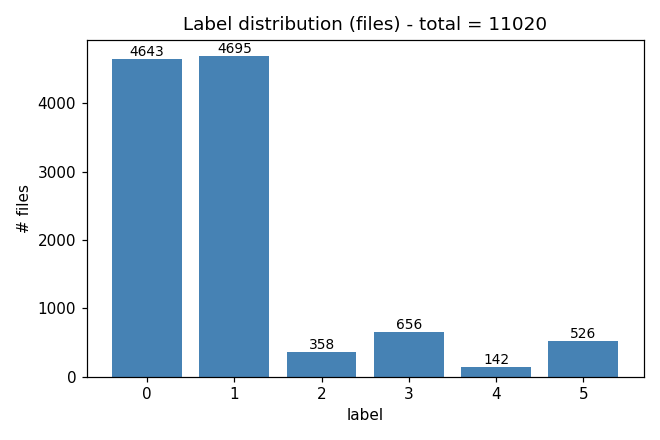
\includegraphics[width=0.78\linewidth]{figures/label-distribution.png}
\caption{Per-file label distribution in the training set. Classes 0 and 1 dominate;
2, 4 and 5 are rare.}
\label{fig:dist}
\end{figure}

\textbf{Naive baseline.} As a reference, I aggregated each file to 12 features (the
time-mean and time-std of the six columns) and trained logistic regression and a
random forest~\cite{pedregosa2011scikit} under the same \texttt{GroupKFold(user)}
setup. The better of the two reached macro-F1~$=0.628$. Its failure pattern was
informative: the frequent classes were already easy, and beating the baseline
required modelling \emph{when} motion happens during the window, not just its
averages.

\section{Preprocessing and Feature Engineering}
Because the data is already aggregated to one-second rows, classical preprocessing
is light: parquet caching, per-fold standardisation for the neural models (the
scaler is fit on the training fold only, to avoid leakage), and class-balanced
sample weights so the rare classes are not ignored. The main effort is per-file
feature construction: I build \textbf{334 features in 17 named groups} (basic
statistics, percentiles, skew/kurtosis, FFT band energy with spectral entropy and
dominant frequency, mean-crossing rates, signal magnitude and signal-magnitude-area,
cross-axis correlations and ratios, jerk, summaries and autocorrelation/peak/tail
statistics of the std channels, temporal-segment statistics, energy and histogram
entropy, and a coefficient-of-variation group).

\textbf{The most valuable change.} Originally the rhythm extractors
(autocorrelation, peak counts, tails) were applied only to the mean channels. The
std channels, however, measure within-second motion intensity, and the rhythm of
that intensity is essentially step cadence. Running the same extractors over the std
channels too is what pushed the leaderboard from the low-0.81 range to 0.8267, even
though it barely moved the cross-validation score. I attribute this to step cadence
being a property of the \emph{activity} rather than of the \emph{person}, so it
transfers to unseen users much better than it appears in same-user validation.

\begin{table}[t]
\caption{Cross-validated macro-F1 (5-fold \texttt{GroupKFold} by user) as each
model class is added on top of the rich features.}
\label{tab:stages}
\centering
\begin{tabular}{lc}
\toprule
Stage / model & CV macro-F1 \\
\midrule
Naive baseline (12 features) & 0.6281 \\
LightGBM~\cite{ke2017lightgbm} & 0.7154 \\
XGBoost~\cite{chen2016xgboost} & 0.7261 \\
CatBoost~\cite{prokhorenkova2018catboost} & 0.7269 \\
MLP & 0.7130 \\
CNN--LSTM (raw signal) & 0.6337 \\
ROCKET (raw signal)~\cite{dempster2020rocket} & 0.6669 \\
\textbf{Final 6-model ensemble} & \textbf{0.7586} \\
\bottomrule
\end{tabular}
\end{table}

Table~\ref{tab:stages} quantifies the effect of each preprocessing/modelling stage.
Feature engineering alone takes the boosted trees from 0.628 to about 0.727, which
is most of the total gain; each additional model family then adds a little, and the
final ensemble reaches 0.7586 in cross-validation. A leave-one-group-out study with
LightGBM (drop one feature group, re-run the full CV) confirmed that no single group
is decisive---the model leans on many correlated views of the signal---while the
basic statistics, percentiles, temporal segments and tails are individually the
strongest.

\section{Aligning Labels with the Time Series}
A file is an ordered sequence of 300 seconds, so a good model must use temporal
structure. I attack this from three complementary angles, chosen so that the models
make \emph{different} errors and therefore combine well.

\textbf{(a) Hand-crafted temporal features.} The most important is normalised
autocorrelation at lags $\{1,2,5,10,20\}$ seconds: a periodic activity (walking)
has high autocorrelation at its stride lag while a static activity has none, giving
a scale-free measure of cadence (and, as noted, it is especially effective on the
std channels). I add FFT band energy and dominant frequency (the frequency-domain
view of cadence), jerk and mean-crossing rates (abruptness and oscillation), and
per-third temporal-segment statistics (how the activity evolves over the window).

\textbf{(b) CNN--LSTM on the raw signal.} I train a sequence model directly on the
raw $6\times300$ input, in the spirit of deep convolutional-recurrent HAR
architectures~\cite{ordonez2016deep}: three 1-D convolution blocks extract local,
shift-invariant motion patterns and downsample the sequence, a two-layer
bidirectional LSTM~\cite{hochreiter1997long} models long-range temporal
dependencies, and time-wise average+max pooling yields a position-invariant
representation. It is trained with class weights, label smoothing, and train-only
augmentation (jitter, circular time-shift, magnitude scaling), with test-time
augmentation at inference. Alone it scores only $\approx0.634$, but its errors are
very different from the trees, which is exactly why it helps the ensemble.

\textbf{(c) ROCKET.} ROCKET~\cite{dempster2020rocket} convolves the raw signal with
several thousand \emph{random} dilated kernels and summarises each by the proportion
of positive outputs and the maximum, with a linear classifier on top. I added it
because the three tree models all read the same tabular features and were making
correlated mistakes; ROCKET reads the raw signal in a completely different
(random, linear) way, scores $\approx0.667$ alone, and its de-correlated errors lift
the cross-validated ensemble by roughly half a point.

\section{Ablation Study and Results}
\textbf{Combining the models.} I compared a logistic-regression stacker on all
out-of-fold probabilities (CV macro-F1 $=0.7271$) against a hill-climbing weighted
blend~\cite{caruana2004ensemble} that starts from nothing and repeatedly adds
whichever model most improves OOF macro-F1 (CV $=0.7530$). The blend won and is
used; a full weight grid over six models is infeasible, and hill-climbing naturally
down-weights the redundant tree models and leans on the diverse CNN, ROCKET and MLP.

\textbf{Per-class threshold tuning.} After blending I apply a per-class additive
offset, tuned greedily on the CV folds, that shifts the decision boundary for the
hard classes. This is one of the two largest contributors to the final score:
removing it drops the public leaderboard from 0.8267 to 0.811, i.e. it is worth
about $+0.016$ on its own.

\begin{figure}[t]
\centering
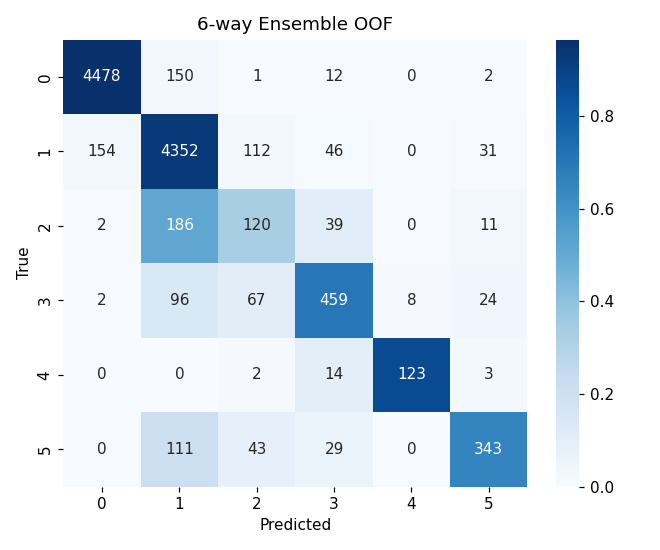
\includegraphics[width=0.74\linewidth]{figures/confusion.png}
\caption{Out-of-fold confusion matrix of the final ensemble. The dominant error is
class~2 being confused with class~1.}
\label{fig:cm}
\end{figure}

\textbf{Where the score is lost.} The per-class F1 of the final ensemble is
$0.97, 0.90, 0.32, 0.73, 0.91, 0.73$ for classes $0$--$5$. Almost all remaining
error is class~2 confused with class~1 (Fig.~\ref{fig:cm}). I verified this is a
genuine ceiling: a classifier trained only to separate class~2 from class~1 still
reaches only $\approx0.78$ AUC, so the two activities look alike from the wrist, and
the tiny class~2 (3\%) is swamped by the huge class~1 (42\%) in the full problem.

\textbf{What did not help (negative ablations).} Documenting failures explains the
final design. The following were implemented, tested, and reverted because they hurt
the public leaderboard relative to 0.8267: orientation-normalised (gravity-aligned)
features (0.8116); multi-scale wavelet-energy features (0.8024); an enriched CNN as a
seventh model (0.8187); a stronger 6000-kernel ROCKET (0.80--0.80); matching the
predicted class balance to the training priors ($0.79$--$0.81$); pushing the class-2
threshold further (0.818, 0.814); and several blend variants---equal weight (0.797),
single best model (0.797), trees only (0.782) and no per-class tuning (0.811).
Pseudo-labelling confident test predictions was rejected after it lowered macro-F1 by
0.011 on held-out users. The clear pattern: once the tree models saturated, neither
recombination nor extra correlated models helped---only genuinely new,
person-invariant signal (the std-channel cadence features) and the per-class tuning
moved the leaderboard.

\begin{table}[t]
\caption{Version history with public-leaderboard macro-F1. ``Kept'' rows build up to
the final submission; ``reverted'' rows are ideas tried afterwards that did not help.}
\label{tab:history}
\centering
\begin{tabular}{llc}
\toprule
Change & Outcome & Public F1 \\
\midrule
Features + LightGBM + CNN + blend & kept & 0.7739 \\
+ XGBoost (3 models) & kept & 0.7919 \\
+ CatBoost + MLP (5 models) & kept & 0.8103 \\
+ ROCKET, hill-climb blend (6 models) & kept & 0.8115 \\
+ std-channel cadence features & \textbf{kept (final)} & \textbf{0.8267} \\
Gravity-aligned features & reverted & 0.8116 \\
Wavelet-energy features & reverted & 0.8024 \\
Enriched CNN (7th model) & reverted & 0.8187 \\
No per-class tuning & reverted & 0.8110 \\
\bottomrule
\end{tabular}
\end{table}

\textbf{Kaggle performance over time.} Table~\ref{tab:history} traces the public
score as the method developed, from the first submission (0.7739) to the final
ensemble (0.8267). The single largest jump came from the std-channel cadence
features, a small and well-motivated feature change rather than additional model
capacity. The per-class one-vs-rest F1 of the constituent models and the ensemble is
shown in Fig.~\ref{fig:pc}; the ensemble matches or exceeds every individual model on
the hard classes.

\begin{figure}[t]
\centering
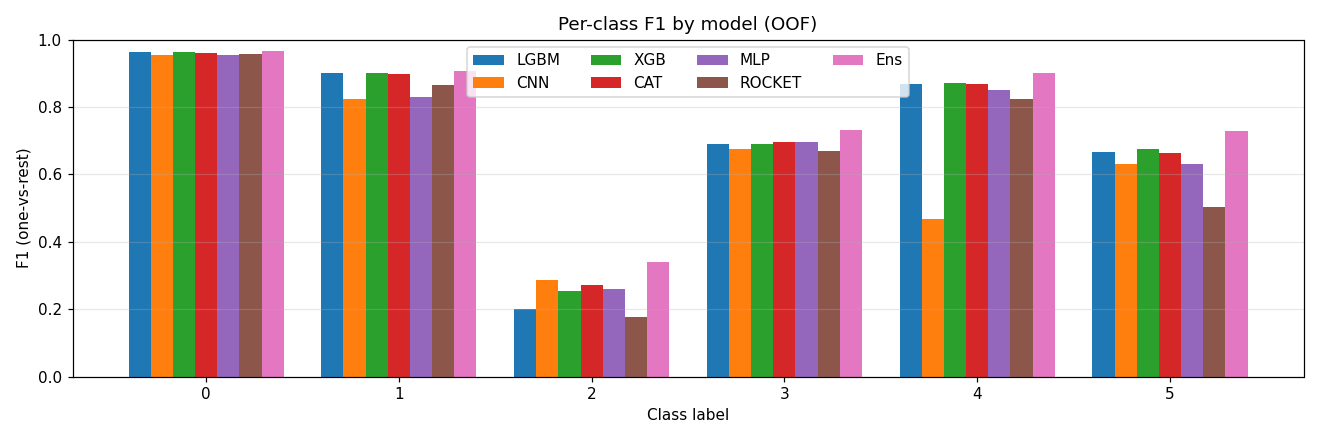
\includegraphics[width=0.95\linewidth]{figures/per-class-f1.png}
\caption{Per-class (one-vs-rest) F1 for each base model and the ensemble (OOF).}
\label{fig:pc}
\end{figure}

\section{Reproducibility}
All code is on the public GitHub repository linked in the abstract. Every random seed
is fixed (\texttt{SEED}~$=42$ for NumPy, scikit-learn, LightGBM, XGBoost, CatBoost and
PyTorch), and every cross-validation split is a \texttt{GroupKFold} on
\texttt{user\_id}. The pipeline can be run in two equivalent ways. (1) Scripts: create
a virtual environment, \texttt{pip install -r requirements.txt} (plus a CPU build of
PyTorch), set \texttt{DATA\_DIR} in \texttt{config.py} to the unzipped Kaggle folder,
and run \texttt{run\_all.ps1}, which executes every stage and writes
\texttt{outputs/submissions/submission\_final.csv}. (2) A single self-contained
notebook, \texttt{HAR\_pipeline\_inline.ipynb}, with every step inlined; its first
cell installs the dependencies, after which all cells run top-to-bottom and produce
the same submission. The notebook has been verified to reproduce the script pipeline
exactly (identical 334 features) and to execute end-to-end without error.

\bibliographystyle{IEEEtran}
\bibliography{reference}

\end{document}
